
% \documentclass[a4paper,twocolumn,sort&compress]{article}
\documentclass[5p,twocolumn,sort&compress]{elsarticle}
% \documentclass[final,5p,times,twocolumn,sort&compress]{elsarticle}
% \documentclass[a4paper,12pt]{report}

\usepackage{amsmath}
\usepackage[binary-units=true]{siunitx}
\usepackage{hyperref}
\usepackage{subcaption}
\usepackage{graphicx}
\usepackage[hmargin=0.5in,vmargin=1in]{geometry}
\usepackage{enumitem}


\sisetup{range-units=single}
\sisetup{range-phrase=\kern 0.08333em--}

\title{Simulating the Measurement of the\\Electron Beam Emittance at AWAKE}
\author{Patrick~Chin}
% \author[ucl]{P.~Chin}
% \author[ucl]{E.~Simpson~Dore}
% \author[ucl]{L.~Deacon}
% \author[ucl]{F.~Keeble}
% \author[ucl]{S.~Jolly}
% \author[ucl]{M.~Wing}
% \address[ucl]{UCL, Gower Street, London WC1E 6BT, UK}
\date{\today}

\begin{document}

\maketitle
\clearpage

\twocolumn[
	\begin{@twocolumnfalse}
		\begin{abstract}
			% In preparation for the experiments at AWAKE, simulations were used to
			% determine to what precision the spectrometer is to be able to measure the
			% emittance of the accelerated electron beam. A range of experimental
			% parameters, including bunch size, energy, energy spread, emittance were
			% tested and the degree to which these parameters effect the measurement of
			% the emittance were determined. Systematic errors arising from the discrete
			% pixels on the screen were found to increase the measurement emittance by
			% \SI{1e-8}{\meter\radian}.
		\end{abstract}

		% \begin{keyword}
		% 	plasma wakefield \sep
		% 	spectrometer \sep
		% 	emittance \sep
		% 	electron beam \sep
		% 	self-modulation instability
		% \end{keyword}
	\end{@twocolumnfalse}
]

\clearpage
\tableofcontents


\section{Introduction}

Advancements in quantum and particle physics are primarily driven by
experimental observations which can verify or refute previous hypotheses, or
can provide data from which new hypotheses can be drawn. 
% This allows us to have a deeper understanding of the universe around us.
Particle colliders are a main source of observational data at the quantum
scale, and can create millions of collision events every second.

%TODO
% Improvements to these colliders come in the form of increasing the luminosity
% of the beam.  beam energy come largely in the form of increasing the energy
% of the colliding particle beams.

Proton--proton beam energies at the Large Hadron Collider (LHC) have recently
reached energies of \SI{13}{\tera\electronvolt} \cite{o2015first}, whereas
lepton--lepton colliders have yet to reach the \si{\tera\electronvolt} energy
scale. The largest of which, the Large Electron-Proton Collider (LEP), was
closed down to make way for the LHC in \num{2000} after having reached a
maximum energy of \SI{209}{\giga\electronvolt} \cite{Barate2003sz}.

\begin{itemize}
	\item reasons why lepton collisions are cleaner than protons
	\item drawbacks of circular accelerator synchrotron radiation at LEP
		\cite{Brandt2000xk}
	\item ICL and CLIC proposed linear RF accelerators ten times larger
		than SLAC
\end{itemize}

% however protons are
% not fundamental particles meaning the energy of each constituent particle is
% less than that of the beam. Leptons however, are fundamental point-like
% particles meaning their centre-of-mass energy can be determined to a higher
% precision and also the collision environment will be much cleaner.

% Looking at current accelerators, circular electron or positron accelerators are
% not possible at these energies unless the accelerator reaches the
% \SI{100}{\kilo\meter} scale as electrons at this energy approach the speed of
% light and since they are accelerating in a circle they will radiate large
% amounts of their energy.
% % \cite{sokolov1966synchrotron}
% An accelerator at the \SI{100}{\kilo\meter} scale is
% impractical due to geographical and financial limitations.  Similar problems
% also arise in linear colliders where current radio-frequency (RF) cavities in a
% linear collider will have to be tens of kilometres in length to reach the
% \si{\tera\electronvolt} scale, this is with current acceleration gradients of
% up to \SI{100}{\mega\volt\per\meter}.  This urges the development of a new
% methods for the acceleration of particles.

The CLIC and ICL are promising proposals for lepton--lepton colliders to reach
the \si{\tera\electronvolt} scale, however

continuing to increase the energy of colliding beams allows for an increasing
number of interactions to be observed.

\section{Proton Driven Plasma Wakefield Acceleration}

Current radio-frequency (RF) accelerator technology is limited to an
electromagnetic gradient of about \SI{100}{\mega\electronvolt\per\meter} due to
RF beakdown.  The ability of plasma to sustain very large 

The concept of accelerating particles in plasma was promising as plasma is able
to sustain large electric fields.  The idea being that energy can be
transferred to a group of charged particles by injecting them into the plasma
wakefield that follows a high energy laser pulse or proton bunch, using the
plasma as an energy transfer medium.  The witness bunch is then accelerated by
the high electromagnetic gradient.

\section{AWAKE}

\subsection{Self-modulation instability}

The first challenge in the development of this accelerator was getting the
length of the proton driver bunch small enough so that resonance occurs with
the electrons in the plasma.  Typical proton bunches, i.e. those produced by
the CERN Super Proton Synchrotron (SPS), have lengths of \(\sim
\SI{10}{\centi\meter}\) which cannot directly create strong plasma waves at the
required wavelength in the \si{\milli\meter} scale as the Fourier component of
the proton beam at the plasma frequency is negligible.
Simulations~\cite{kumar2010self} on the compression of these bunches show that
reducing the longitudinal phase volume blows up the transverse phase volume.
An alternative method would be to split up the proton bunch into a number of
micro-bunches to be simultaneously decelerated.

An instability between the beam and the plasma arises from the mutual
amplification of the rippling of the beam radius and the plasma wave. This
instability tends to destroy the plasma wave as the amplification focuses and
defocuses selected slices of the beam.  This problem was solved by seeding the
self-modulated instability (SMI) with a short electron bunch
\cite{lotov2013natural}, a laser pulse \cite{siemon2013laser} or a sharp cut in
the bunch profile\cite{kumar2010self}. This will promote a single mode and
suppress other modes, including the strongest competing modes, the hosing modes
\cite{vieira2014hosing} and produce well-separated micro-bunches.

\subsection{Uniform-density plasma cell}

The plasma wavelength is \(\lambda_{pe} \approx \SI{1.26}{\milli\meter}\)
meaning that the \SI{10}{\centi\meter} proton bunch will have to be split into
\(\sim 100\) micro-bunches in order to be able to drive the wake.  Each
micro-bunch contributes to the wakefield, and only if the plasma density is
uniform will the contribution of each bunch be coherent. Incoherence will cause
the electron bunches to arrive at the wrong phase in the plasma oscillation. An
increase in the plasma density will shorten the plasma wavelength causing the
electron bunch to crest plasma wave it was riding and fall into the defocusing
phase of the plasma wave as shown in Fig \ref{fig:phases}(a). A decrease
in the plasma density will increase the plasma wavelength causing the plasma
wave to fall further behind the electron bunch meaning the electron bunch to
fall into the trough of the plasma wave resulting in a deceleration of the
electron beam \ref{fig:phases}(c). The electron beam must be in the
region of length \(\lambda_{pe}/4\) between the defocusing and decelerating
phases of the plasma wave.
% These effects are significantly larger for the electrons as protons have
% large longitudinal momentum.

\begin{figure}[tb]
	\centering
	\begin{subfigure}{\linewidth}
		\centering
		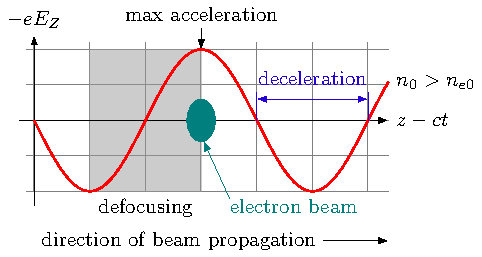
\includegraphics[width=0.9\linewidth]{figures/phases-a.pdf}
		\caption{asdkfjasdlfj sdk dfs f}
	\end{subfigure}
	\begin{subfigure}{\linewidth}
		\centering
		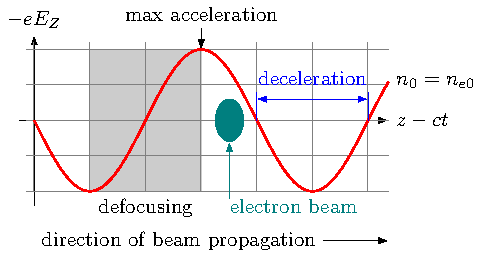
\includegraphics[width=0.9\linewidth]{figures/phases-b.pdf}
		\caption{asdkfjasdlfj sdk dfs f}
	\end{subfigure}
	\begin{subfigure}{\linewidth}
		\centering
		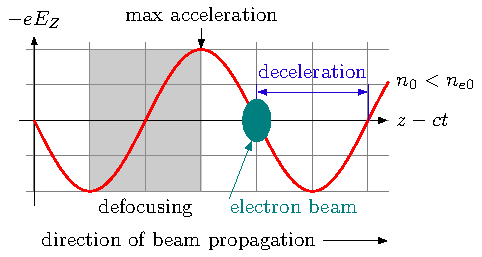
\includegraphics[width=0.9\linewidth]{figures/phases-c.pdf}
		\caption{asdkfjasdlfj sdk dfs f}
	\end{subfigure}
	\caption{
		Phasing of the electron bunch for increased density (a) correct density
		(b) and decreased density (c). \cite{wiedemann2007particle}
	}
	\label{fig:phases}
\end{figure}

This requirement of the plasma limits the plasma selection to being uniform
rubidium vapor, ionised by a co-propagating laser pulse \cite{oz2014novel,
oz2014bja}.  Rubidium was chosen due to it's low ionization potential and heavy
atomic mass.  A heavy element is required to minimize the movement of the
plasma's nuclei which causes adverse effects on the plasma's behaviour
\cite{vieira2012nj, vieira2014bqa}. The Rubiduim vapor is kept in thermodynamic
equilibrium at a constant temperature and volume.

\subsection{Injection of the witness beam}

Due to SMI, the shape of the drive beam changes in the plasma and for the first
four meters, the difference between the phase velocity of the wakefield and the
proton beam velocity is quite large and this will effect the electron beam in
the same manner as having a non uniform plasma, detailed above. To avoid this
problem it was suggested that the electrons could be injected into the plasma
after SMI had fully developed. The design of the injection method arrived at
passing the electron beam through a narrow vacuum tube separated from the
plasma by a thin foil. Then after \(\sim \SI{4}{\meter}\) the electrons will be
directed into the wakefield close close behind the proton driving beam.

\subsection{AWAKE}

The aim of this experiment is to provide a proof of concept for proton driven
plasma wakefield acceleration.  An overview of the experiment is as follows:

The SPS will provide the \SI{400}{\giga\electronvolt} proton driver beam with a
bunch length of \(\sigma_z = \SI{12}{\centi\meter}\) and an intensity of \(\sim
3\times 10^{11}\) protons/bunch. This will travel down the \SI{750}{\meter}
long CNGS transfer line and be focused to \(\sigma_{x,y} =
\SI{200}{\micro\meter}\) and enter a \SI{10}{\meter} long Rubiduim vapor plasma
cell with an adjustable density at the \(10^{14}\) to \(10^{15}\)
electrons/\si{\per\centi\meter} scale.

The proton driver will self modulate at the plasma wavelength \(\lambda_{pe}\)
after being seeded by a high powered \(\approx \SI{4.5}{\tera\watt}\) laser
pulse that is co-axial and co-propagating with the proton driver beam. This
laser also serves the purpose of ionising the Rubidium vapor. These two beams
need to be synchronous to within \SI{100}{\pico\second} and the focal point of
the proton beam is required to be \(\le\SI{100}{\micro\meter}\) and
\(\le\SI{15}{\micro\radian}\) so they are co-axial for the full length of the
plasma cell.

The electron witness beam will be created via photo-emission by an illuminating
cathode electron source and accelerated by a 2.5 cell RF-gun and a meter long
booster at \SI{3}{\giga\hertz}.

%TODO injection

\section{Project outline}

% \lipsum[3-10]

The development of this experiment has been heavily simulation driven.
Simulation code developed specifically for the simulation of the plasma to be
able to resolve for time scales of \(\omega_p^{-1}\), (where \(\omega\) is the
frequency of the plasma wave) and length scales of down to \(c/\omega_p\), as
existing codes were not tuned to resolve at these scales.  Different simulation
softwares are tuned to be used for different sections of the AWAKE experiment.

% I will be working on simulating the electron spectrometer using
% BSDIM~\cite{agapov2009bdsim}, simulation software in active development,
% designed to simulate and track particle beams passing through accelerators and
% detectors. It is built on top of the Geant4
% toolkit~\cite{agostinelli2003geant4} for the simulation of particles through
% matter, which also provides the graphical user interface for a visualisation of
% the simulation.  Event data is stored using ROOT~\cite{antcheva2011root}, an
% advanced statistical analysis and visualisation framework designed to work for
% petabyte scale data storage.

% More specifically, I will initially be looking at calculating the emittance of
% the accelerated electron beam using data from simulated accelerated electron
% beams.  Recent simulations of the spectrometer used an idealised electron beam
% \cite{deacon2016qjq} and I will be continuing this line of investigation.  The
% electron beam profile and other properties immediately after it leaves the
% plasma cell will be provided by separate simulations using LCODE.  This data is
% used as input for the BDSIM simulation where we will simulate the beam passing
% through dual focusing quadrupoles in both the horizontal and vertical planes.
% The simulation will be able to provide all the raw data about the final state
% of the electron beam, however, in reality we will not be able to simply query
% the beam properties. The measurement of the energy spectrum will be carried out
% by using a magnetic dipole downstream of the dual quadrupoles, and observing
% the horizontal spread of the electron beam on a screen. This screen will also
% be sumulated with BDSIM taking into account the screen resolution and detection
% rates.

% I will also be working on the modeling and simulation of the background
% radiation from the plasma cell and other sources using real world data to help
% build an accurate model.  All of these simultions along with real data will
% help in finding optimal parameters for each component of the spectrometer,
% including the strength of the quadrupoles and the dipole, the lens parameters
% of the camera and the properties of the screen.



\section{Theory}

% \section{Single Particle Dynamics}
% \label{sec:single_particle_dynamics}

% To derive the method used in simulating the beam, it is usefull to start with
% Maxwell's equations. These can be used to describe the motion for charged
% particles under the magnetic fields of accelerator components, such as dipoles
% and quadrupoles. The solutions to these equations become increasingly complex at
% higher perturbations so it is usefull to devise a coordinate system other than

% Specifying a coorindate system such that the origin follows the ideal path of
% the particle beam, rather than a coordinate system about an arbitary fixed
% point we are able to describe the state of a patricle by

% \begin{equation}
% 	\begin{pmatrix}
% 		x(z) \\ x'(z) \\
% 		y(z) \\ y'(z) \\
% 	\end{pmatrix}
% 	=
% 	\begin{pmatrix}
% 		C_x(z)  & S_x(z)  & 0 & 0 \\
% 		C'_x(z) & S'_x(z) & 0 & 0 \\
% 		0 & 0 & C_y(z)  & S_y(z)  \\
% 		0 & 0 & C'_y(z) & S'_y(z) \\
% 	\end{pmatrix}
% 	\begin{pmatrix}
% 		x_0 \\ x'_0 \\
% 		y_0 \\ y'_0 \\
% 	\end{pmatrix}
% \end{equation}

% where \(x\) and \(y\) are deviations form the centre of the beam along their
% respective axis and \(x'\) and \(y'\) are the transverse momenta of the
% particle perpendicular to \(z\), the direction of travel of the beam.
% Transformations in either the $x$ or $y$ plane are independent, however, it is
% clear that coupling effects can still be included
% % TODO

\subsection{Single Particle Dynamics}

When working with beams of particles, it is advantagous to work in the
coordinate system that follows the ideal path of the beam. If the beam's motion
in the \(x\) and \(y\) planes are independent, i.e. we ignore coupling terms,
the each particle's motion in each plane can be described by
\begin{equation}
	\begin{pmatrix}
		u(z) \\ u'(z)
	\end{pmatrix}
	=
	\begin{pmatrix}
		C_u(z)  & S_u(z)  \\
		\sqrt{C'_u(z)} & S'_u(z)
	\end{pmatrix}
	\begin{pmatrix}
		u_0 \\ u'_0
	\end{pmatrix}
\end{equation}
where \(u\) is either \(x\) or \(y\) and \(u'\) is the transverse velocity of
the particle in the \(u\) plane. The coordinate \((u, u')\) lies in what is
known as phase space. Using this system of matricies the drift and quadrupole
matricies can be derived \cite{wiedemann2007particle}. The drift matrix is
\begin{equation}
	\mathcal{M}_D(l) =
	\begin{pmatrix}
		1 & l \\
		0 & 1
	\end{pmatrix} \\
\end{equation}
the focusing quadrupole matrix is
\begin{equation}
	\mathcal{M}_{QF}(l) =
	\begin{pmatrix}
		\cos\psi & \frac{1}{\sqrt{k}}\sin\psi \\
		-\sqrt{k}\sin\psi & \cos\psi
	\end{pmatrix} \\
\end{equation}
and the defocusing quadrupole matrix is
\begin{equation}
	\mathcal{M}_{QD}(l) =
	\begin{pmatrix}
		\cosh\psi & \frac{1}{\sqrt{\abs{k}}}\sinh\psi \\
		-\sqrt{\abs{k}}\sinh\psi & \cosh\psi
	\end{pmatrix}
\end{equation}

These transport matricies can be multiplied together resulting in the
transformation matrix representing a path containing all accelerator components
making it simple to follow a particle through a transport line.

\subsection{Emittance}

\begin{figure}
	\centering
	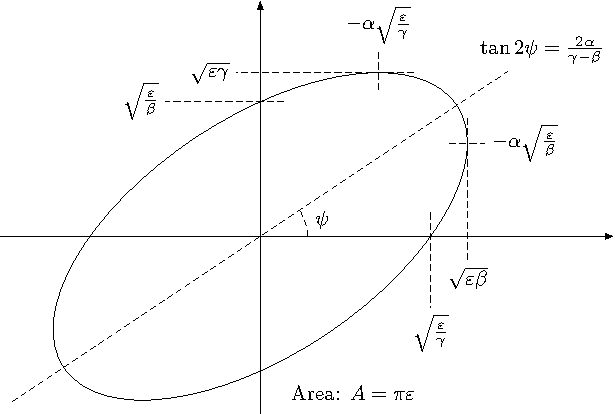
\includegraphics{figures/ellipse}
	\caption{
		A representation of the relation between the Twiss parameters of
		a beam's ellipse in phase space~\cite{wiedemann2007particle}.}
	\label{fig:ellipse}
\end{figure}

Grouping the individual particles in a particle beam, they will occupy an area
in phase space known as the emittance.  Qualitatively the emittance of a beam is
a measure of how parallel the particles of the beam are to each other. It is a
conserved quantity while the beam is not being acted upon by external forces.

In phase space the beam of particles will usually take up an area resembling
that of an ellipse. This is because, after a diverging or converging beam has
traveled through an apeture, we expect particles that are further away from the
centre of the beam to have a larger transverse momentum. This is unless the beam
is being measured at it's waist where it is transitioning between converging and
diverging or visa versa. Figure~\ref{fig:ellipse} shows the projection of a
diverging beam onto a two dimensional phase plane, called the phase ellipse.
The line that defines the ellipse is drawn such that \SI{95}{\percent} of all
the particles in the beam are contained~\cite{buon1994beam}. The emittance is
defined by the area of this ellipse divided by \(\pi\) in units of
\si{\meter\radian}. Note that in general the transverse momenta, hence the slope
of the particles in the beam, are very small so the approximation \(\sin
u'\approx u'\) can be used.

% \begin{equation}
% 	\int_{\text{ellipse}}\mathrm{d}x\mathrm{d}x' =\pi\epsilon
% \end{equation}

The general equation of an ellipse can be used to describe the phase ellipse:
\begin{equation}
	\gamma x^2 + 2\alpha xx' + \beta x'^2 = \epsilon
\end{equation}
where \(\alpha\),  \(\beta\), \(\gamma\) and \(\epsilon\) are ellipse parameters
that determine the ellipse's shape and orientation in phase space, where
\(\epsilon\), the area of the ellipse is the emittance~\footnote{Often, the
units of \(\pi\) are omitted and the emittance is given in units of
\si{\pi\;\meter\;\radian}.} Of the four beam parameters, only three are
independant and since \(\epsilon\) is defined as the area, the other three can
be found to be correlated from the ellipse's geometric properties by
\begin{equation}
	\beta\gamma - \alpha^2 = 1
\end{equation}

% \subsection{Methods of measurement}

% The phase-space density and emittance of a beam must be infered from beam
% profiles captured using charge-coupled device (CCD) cameras after undergoing
% spatial filtering.

By expressing this ellipses as a matrix, transformation rules have been derived
to transport the beam~\cite{wiedemann2007particle}. The beam matrix can be
defined by
\begin{equation}
	\bm{\sigma} =
	\begin{pmatrix}
		\sigma_{11} & \sigma_{12} \\
		\sigma_{21} & \sigma_{22} \\
	\end{pmatrix}
	=
	\epsilon
	\begin{pmatrix}
		\beta & -\alpha \\
		-\alpha & \gamma \\
	\end{pmatrix}
\end{equation}
where each element describes distributions of particles in the beam as follows:
\begin{align}
	\sigma_{11} &= \langle x_i^2 \rangle = \epsilon\beta \\
	\sigma_{22} &= \langle {x'}_i^2 \rangle = \epsilon\gamma \\
	\sigma_{12} &= \langle x_i x'_i \rangle = -\epsilon\alpha
\end{align}

The evolution of this matrix along the beam transport line can then be described
by
\begin{equation}
	\bm{\sigma}_1 = \mathcal{M}\;\bm{\sigma}_0\;\mathcal{M}^T
	\label{eq:apply}
\end{equation}

% TODO measurement of the emittance 183gg (page 164)

\section{The Simulation}
\label{sec:simulation}

\begin{table*}[!tb]
	\centering
	\begin{tabular}{ll}
		\toprule \midrule
		Parameter & Value \\ \midrule \midrule

		Screen and Camera \\ \midrule
		Screen width & \SI{1}{\meter} \\
		Screen height & \SI{65}{\milli\meter} \\
		% % FOV 1.149
		Horizontal pixels & 1850 \\
		% % optical point spread function set to 0?
		% % width of x sensor? \SI{25e-3}{\metre}
		Screen efficiency & \SI{5000}{photons\per electron}\\
		Camera acceptance & \num{1.5e-5} \\
		Camera MCP Gain & 1442 \\
		Camera quantum efficiency & 0.15 \\

		\midrule
		Accelerated electron beam \\ \midrule
		Emittance \(\left(\epsilon\right)\) & \SI{1e-6}{\meter\radian} \\
		% Beam size parameter \(\left(\beta\right)\) & \SI{1}{\meter} \\
		\(\beta\) & \SI{1}{\meter} \\
		\(\alpha\) & \SI{0.5}{\radian} \\
		Mean energy \(\left(\bar{E}\right)\) & \SI{1.3}{\giga\electronvolt} \\
		Energy spread \(\left(\sigma_E\right)\) & \SI{0.4}{\giga\electronvolt} \\
		Electrons/bunch \(\left(N_{e^-}\right)\) & \num{1e9} \\
		% \(N_{e^-}\) & \num{4e8} \\
		Background photon density & \SI{3.415e4}{\per\meter\squared} \\
		% Thermal electrons \(N_{e^-_\text{thermal}}\) & \SI{0.016}{\per\second} \\
		\bottomrule
	\end{tabular}
	\caption{
		The expected values for many experimental parameters have been
		calculated.
		% It should be noted that these values are missing error
		% values. It can be assumed that the error on each value can be given by
		% half the least significant digit.
	}
	\label{tab:expected}
\end{table*}

The simulation of this experiment was split into three parts: the simulation of
the beam, the simulation of the effects of the background and camera, and the
reconstruction of the beam to measure the parameters of the beam.

\subsection{The Electron Beam}

% TODO explain LCODE electrons (cite)

Given enough computing power and time, the simulation of the beam from, the end
of the plasma cell, passing through two quadrupoles and through a dipole could
have been done on BDSIM~\cite{agapov2009bdsim}, a
Geant4~\cite{agostinelli2003geant4} toolkit for simulating radiation traveling
through an accelerator. This software package simulates a each particle
individually, updating it's position and velocity at each step through the
accelerator by applying the effect of forces from all fields within the
accelerator.  For beams consisting of \num{\sim e9} particles, tracking each
particle individually as they travel down the beam line would take enormous
amounts of time and available computing power, and as many simulations were
required to be performed this would have been impractical for obtaining any
reasonable amount of data.

A new program was written, taking advantage of beam matrices to describe the
beam as a whole. The goal of the first part of this program is to simulate the
intensity of the incident beam at each pixel on the screen.

\subsubsection{BDSIM Calibration}

\begin{figure*}[!tb]
	\centering
	\begin{subfigure}[t]{\columnwidth}
		% 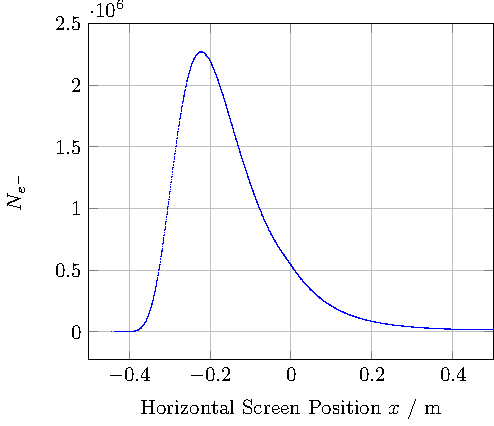
\includegraphics[width=1\linewidth]{./figures/edist.pdf}
		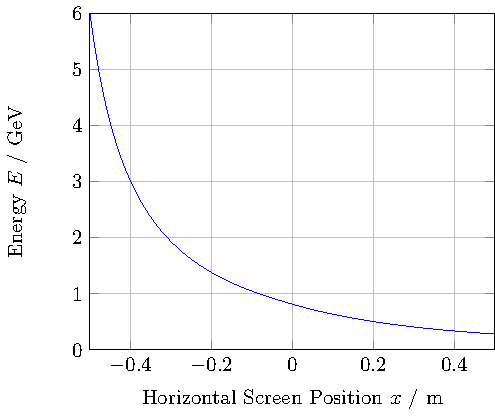
\includegraphics{./figures/eofx.pdf}
		\caption{
			Electron energies corresponding to the horizontal screen position
			due to the effect of the dipole.
		}
		\label{fig:eofx}
	\end{subfigure}\hfill~
	\begin{subfigure}[t]{\columnwidth}
		% 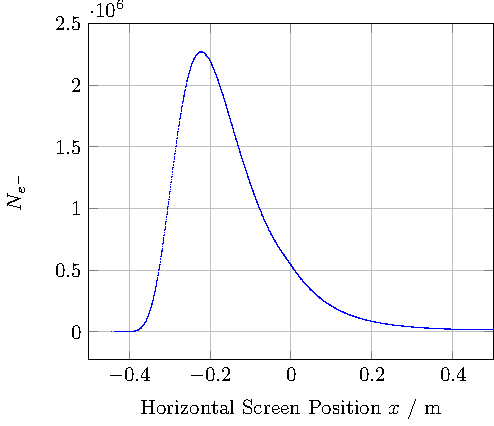
\includegraphics[width=1\linewidth]{./figures/edist.pdf}
		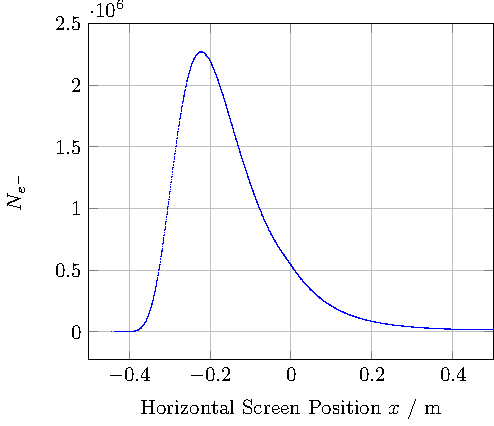
\includegraphics{./figures/edist.pdf}
		\caption{
			The number of electrons expected to hit the screen at each \(x\)
			position for \(E=\SI{1.3}{\giga\electronvolt}\) and
			\(\sigma_E=\SI{0.4}{\giga\electronvolt}\).
			% other experimental parameters are set to their expected values.
		}
		\label{fig:edist}
	\end{subfigure}
	\caption{
		The functions \(E(x)\) and \(N_{e^-}(x)\) extracted from the BDSIM
		calibration output data. These functions are used to calculate the
		horizontal spread of the electrons across the screen.
	}
\end{figure*}

The effect of the quadrupole and the dipole are dependant on the energy of the
individual electrons in the beam.  So to calculate the density of an electrons
along with their energies as a function of the horizontal screen position a
number of BDSIM simulations were run. \num{e5} electrons where fired
individually down the simulated AWAKE beam line. These electrons had a square
energy distribution from \SIrange{0}{10} {\tera\electronvolt}, and had a
Gaussian spacial distribution with \(\sigma_x = \sigma_y =
\SI{6}{\milli\meter}\), and no transverse momentum hence zero emittance. This
large energy range was chosen as to encompass the entire energy range that would
hit the screen. The dipole was set to it's highest setting of \SI{650}{\ampere}
to achieve the maximum spread of the beam on the screen.

% TODO why use no emittance beams for calibration
These BDSIM runs were used to plot the function in Figure~\ref{fig:eofx} which
shows the relationship between the electron energy and where is it expected to
hit the screen. Figure~\ref{fig:edist} is an example of the horizontal
distribution of a beam of electrons with a Gaussian energy spread onto the
screen. This was calculated by applying the inverse of the function \(E(x)\)
shown in Figure~\ref{fig:eofx}, to the energy distribution of the beam.

At these experiment settings, the entire of the beam electrons hit the screen
allowing for a more accurate measurement of the beam parameters.  The effect of
the emittance and quadrupoles on the horizontal spread is taken to be negligible
in comparison to the effect of the dipole, and so it's effect is taken into
account by adding a horizontal smearing to the horizontal position of each
electron on the screen. This results in this plot being all that is required to
simulate the transverse spread of the beam.

The drift distances from the second quadrupole to the screen were also recorded
for each \(x\) position on the screen. This function \(d(x)\) is used in the
calculation of the vertical beam size, discussed next.

% Since the effect of the dipole on the beam depends on the energy of each
% individual particle, the evolution of the beam through the dipole cannot be
% calculated reasonably using beam matrices. So, to simulate the dipole, 

\subsubsection{Deriving the Beam Size Function}

The dipole spreads the beam horizontally across the screen. The electrons in
each vertical strip of pixels are grouped together and their energy approximated
to be equal. This is allowed as the energy spread in each strip will always be
less than \SI{0.5}{\percent}. This was calculated from data used to plot
Figure~\ref{fig:eofx}, by finding the ratio between the difference in energies
between adjacent strips, by the energy value at that strip. This was done for
all strips and the maximum value was a \SI{0.5}{\percent} difference in energy.

Using this assumption, we are able to create one beam and transport matrix for
electrons in each vertical stream of pixels. The root mean square of the
vertical beam size on the screen can be extracted from the resultant beam matrix
\(\sigma_1\). To arrive at this beam matrix, the transport matrix
\(\mathcal{M}\) is applied to the initial beam matrix \(\sigma_0\) in
(\ref{eq:apply}). The transport matrix is the product of the transport matrices
of each component of the spectrometer:
\begin{equation}
	\begin{split}
		\mathcal{M} = \mathcal{M}_D(d) \cdot \mathcal{M}_{QD}(l_2) \cdot
		\mathcal{M}_D(g_2) \\
		\cdot\;\mathcal{M}_{QF}(l_1) \cdot \mathcal{M}_D(g_1)
	\end{split}
\end{equation}
where \(\mathcal{M}_D(d)\) is the drift transport matrix which is a function of
the travel distance and \(\mathcal{M}_{QD}(l)\) is the transport matrix of the
quadrupole. \(g_1\) is the drift distance (the gap) between the end of the
plasma cell and the first quadrupole, \(g_2\) is the gap between the two
quadrupoles, \(l_1\) and \(l_2\) are the effective quadrupole lengths of the
focusing and defocusing quadrupoles respectively. \(d\) is the drift distance
between the second quadrupole and the screen, taking into account the effect of
the dipole, hence, is a function of the energy. The shape of this function was
calculated in the BSDIM runs.

For simplicity, it is assumed that the quadrupoles strengths \(k_1\) and \(k_2\)
are set to values such that each quadrupole focuses at the mean energy of the
beam, hence these variables are proportional to the beam's mean energy.

% TODO why is the first gap not taken into account? or why it equal zero
% how are the quadrupole lengths calculated?

% The beam matrix element \(\sigma_{11} = \langle y \rangle^2 = \epsilon\beta\)

Applying the matrix multiplication results in the vertical beam size as a
function of the horizontal screen position:
\begin{equation}
	\begin{split}
		\sigma_y^2 = \sigma_{1,11} =\: & C^2(x)\sigma_{0,11} \\
									&+ 2C(x)S(x)\sigma_{0,12} \\
									&+ S^2(x)\sigma_{0,22}
	\end{split}
\end{equation}

After generating, a two dimensional histogram representing the number of
electrons hitting the screen at each pixel the goal is to simulate the
effectiveness of the equipment and translate this number to represent the raw
signal that will be read off for each pixel.

\subsection{Backgrounds}

How good the measurement of the emittance is, is most dependant on the magnitude
of the multiple sources of backgrounds as well as the reliability of the
equipment. The following sources of error were taken into account: the
efficiency of the scintillator screen, the acceptance of the camera due to it's
distance from the scintillator screen, the background photon density, the
emittance of photoelectrons in the camera, the thermal noise in the camera, the
amplification by the microchannel plate (MCP) and the readout noise.  Each
source of noise is added to each pixel independently.

% TODO ask about the acceptance value.
% do we assume scintillator emits photons evenly?
% how far is the camera from the screen - I should know this
% what is the acceptance of the camera?
% where does the value 1e5*64/80 come for the background photon density?
% where do we assume the background photon density comes from

% TODO cite 5000
The first two error sources, the scintillator screen and the camera acceptance,
both scale the signal. So for each electron that hits the screen, it is
expected that an average of \num{5000} photons are to be emitted. The
camera acceptance, is the ratio of photons that the camera registers to the
number of photons emitted by the scintillator, with a value of \num{1.5e-5}.
After the addition of these two effects, the camera is expected to receive
\SI{7.5}{\percent} of the original electron signal. The expected value for the
number of photons incident on the camera due to the beam electrons is a Poisson
random number.

It is assumed that there is a uniform distribution of photons incident on the
camera. The density of these electrons is expected to be
\SI{3.415e4}{photons\per\meter\squared} equating to \num{0.01} background
photons per pixel during the \SI{3e-3}{\second} the gate is open. The number of
background photons that hits a pixel is a discrete value, and so is also
generated by generating a Poisson random number.  As discussed later in
Section~\ref{sec:results} this value is very small in comparison to the signal
produced by the beam and will only have an effect if the density of background
photons is multiple magnitudes larger than the expected value.

The camera's photomultipliers then convert the photons of light back to an
electrical current. This multiplies the incident number of photons by the
quantum efficiency of the camera, \num{0.15}. % TODO cite The expected number of
thermal photoelectrons per pixel per second is expected to be
\num{0.016}~\cite{istarscmos}, with the camera running at the expected
temperature of \SI{-30}{\celsius} with \SI{16}{\celsius} cooling water and an
ambient room temperature of \SI{16}{\celsius}. This value is typically doubles
for each \SI{5}{\celsius} rise in temperature of the camera \cite{istarscmos}.
At these running temperatures of the camera, about 9 photoelectrons are expected
to be generated during the time the gate is open, which is an insignificant
proportion in comparison to the beam signal, creating \num{1e7} photoelectrons
before MCP amplification.

% TODO lookup Intensified CCD Cameras
The microchannel plate amplifies the number of photoelectrons by \num{1442},
also amplifying all previously added backgrounds as well. This was simulated by
scaling the value of the bin, and it's error, by \num{1442} rather than
generating a Poisson random number. The modelling of this process may not be
reflect the true nature of this process due to an uncertainty in underlying
process, however the overall effect remains accurately simulated. Despite this,
the error arising from this process is likely to scale the error as mentioned.
% TODO why is a Poisson number not generated for MCP?

And finally, before the values of the signal is obtained, a readout noise is
added. This background is expected to add \num{7.2} readout electrons per image
pixel for the camera operating at \SI{1}{\mega\hertz}.
% TODO see camera description for the readout noise

\subsubsection{Error Calculations}

Poisson statistics were used for the calculation of errors.  Once the shape of
the incident beam on the screen was calculated the number of electrons incident
on each pixel was given an error of the square root of the count. Two methods of
error propagation were used depending on the nature of the process involved.
The following processes were modeled as additive processes: background photons
hitting the screen, the thermal electrons from the currents in the camera and
the readout noise, whereas the multiplicative processes are: photon generation
at the scintillator screen, photoelectron generation in the camera PMTs and the
amplification of the electron signal by the MCP.

Basic error propagation techniques were used here. For the additive processes,
where the new value of each bin $n$ is the sum between the old bin value $n_0$
and the value given by the process $n_\text{proc}$: $n=n_0+n_\text{proc}$ the
propagation of error is given by calculating the hypotenuse of the absolute
errors:
\begin{equation}
	\Delta n= \sqrt{\Delta n_0^2 + \Delta n_\text{proc}^2}
\end{equation}
where the error of a Poisson random number is the square root of the value.

For the multiplicative processes, i.e. $n = \lambda_\text{proc}n_0 $ where
$\lambda_\text{proc}$ is the scaling factor of the process the propagation of
the error is given by calculating the hypotenuse of the percentage errors:
\begin{equation}
	\Delta n= n \sqrt{
		\left( \frac{\Delta n_0}{n_0} \right)^2 +
		\left( \frac{\Delta \lambda_\text{proc}}{\lambda_\text{proc}} \right)^2}
	\label{eq:error_mul}
\end{equation}

% \begin{equation}
% 	\Delta n= n \sqrt{
% 		\left( \frac{\Delta n_0}{n_0} \right)^2 +
% 	\left( \frac{\sqrt{\lambda_\text{proc}n_0}}{\lambda_\text{proc}n_0} \right)^2}
% \end{equation}

Many of the errors \(\Delta n_\text{proc}\) and \(\Delta \lambda_\text{proc}\)
were unavailable at the time of simulation. All background noises are modeled as
uniformly distributed Poisson random numbers so under these assumptions the
associated error on each value can correctly be taken to be the square root of
the value. % TODO you sure not the sqrt of the mean value?
For multiplicative processes the resultant values were also Poisson random
numbers meaning (\ref{eq:error_mul}) can be rewritten as
\begin{equation}
	\Delta n= n \sqrt{
		\left( \frac{\Delta n_0}{n_0} \right)^2 +
	\left( \frac{\sqrt{n}}{n} \right)^2}
\end{equation}
where the full statistical error of the generated value is taken into account
without knowledge of the error of the scaling factor.
% TODO simply scaling the errors up with the MCP?

\subsection{Calculating the Emittance}

The signal received from the camera is required to be scaled back to represent
the real beam size on the screen. The effect of additive backgrounds and scaling
processes are reverted in the reverse order of their application arriving at a
measured value for the number of electrons that hit the screen at each pixel.

To calculate the vertical beam size for each pixel strip, a Gaussian function is
fitted to the vertical beam profile using CERN ROOT's \(\chi^2\) minimising
fitting algorithm~\cite{Brun:1997pa}.
% TODO gaussian function
The root mean square of the fitted
Gaussian is then calculated for each strip to obtain the vertical beam size at
each horizontal position on the screen. These points are displayed as the black
points in the beam reconstruction plots in Figures~\ref{fig:default}
and~\ref{fig:yoverestimate}.

Finally, the vertical beam size function, previously used to simulate the shape
of the incident electron beam, is then fitted to the measured beam sizes. Again,
the fitting is done wholly using ROOT's \(\chi^2\) minimising fitting algorithm,
where the three beam parameters \(\epsilon\), \(\beta\) and \(\gamma\) as
parameters to be minimised.



\section{Results}
\label{sec:results}

% \subsection{The Output Plot}
% \label{sub:output}

\begin{figure}[!tb]
	\centering
	\includegraphics[width=\columnwidth]{./output/run-bgdens/bgphotons_1/n1/graph.pdf}
	\caption{
		The beam reconstruction (blue line) of a sumlation run with all the
		expected parameter values. \(E = \SI{1.3}{\giga\electronvolt}\),
		\(\sigma_E = \SI{0.4}{\giga\electronvolt}\), \(\epsilon =
		\SI{1}{\milli\meter\milli\radian}\)
	}
	\label{fig:default}
\end{figure}

\begin{figure}[!tb]
	\centering
	% 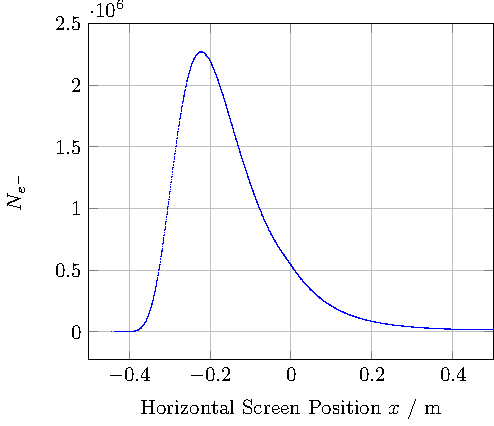
\includegraphics[width=1\linewidth]{./figures/edist.pdf}
	\includegraphics[width=\columnwidth]{./output/run-pespread/pespread_0.01/n1/graph.pdf}
	\caption{
		The beam reconstruction, consistently overestimates the vertical
		beam size. This run used a small percentage energy spread of
		\SI{1}{\percent}. With all other parameters set to their expected
		value.
	}
	\label{fig:yoverestimate}
\end{figure}


Along with the \(\chi^2\) minimised parameter values of the fit, each simulation
generated a plot, showing the simulated, measured and fitted vertical beam size
functions as a function of horizontal position \(x\) on the screen.
Figure~\ref{fig:default} is the output of a run with all parameters set to their
expected values. At these values, the measured beam sizes and the fitted
Figure~\ref{fig:yoverestimate} is an output plot for a run with a small
(\SI{1}{\percent}) energy spread. The solid black line is the shape of the
simulated electron beam that hits the screen, the black points show the
simulated measurements of the RMS width of the fitted gausian for each vertical
strip of pixels. The blue dashed line is the beam size function fitted to the
points.

\subsection{Binning errors}

After the investigation of multiple experimental parameters, the emittance
measurement consistently converged to a value \num{1e-8} larger than the input
emittance. The reason for this systematic error was found to be due to the
discritisation of the beam hitting the screen meaning that the measurement of
the vertical beam size was consistently overestimated. Since the electrons in
each pixel are not uniformly distributed but rather more densely distributed
closer towards the mean value, giving rise to a systematic overestimation of the
vertical beam size of up to two times the vertical size of the pixel. This
effect can be seen most clearly when a very small energy spread was used as can
be seen in Figure~\ref{fig:yoverestimate}, where the measured beam heights are
consistently larger than the actual beam height.

This systematic error is displayed in subsequent plots as a blue line, where the
red line shows the true beam emittance and the blue line represents where the
emittance measurement should be taking into account this error.

\subsection{Energy Spread}

\begin{figure}[!tb]
	\centering
	% 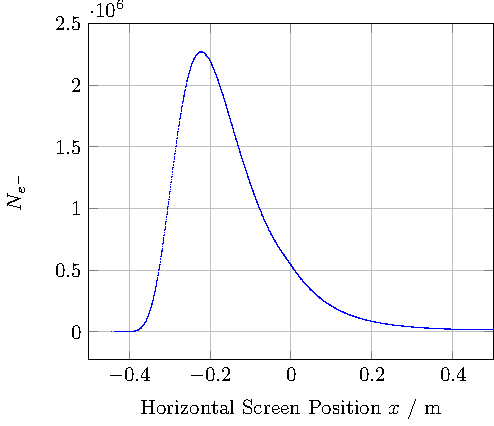
\includegraphics[width=1\linewidth]{./figures/edist.pdf}
	\includegraphics{./output/run-pespread/emit_vs_pespread.pdf}
	\caption{
		Plot of the simulated emittance measurement against the percentage
		spread of beam energy.
	}
	\label{fig:emit_pespread}
\end{figure}

\begin{figure}[!tb]
	\centering
	% 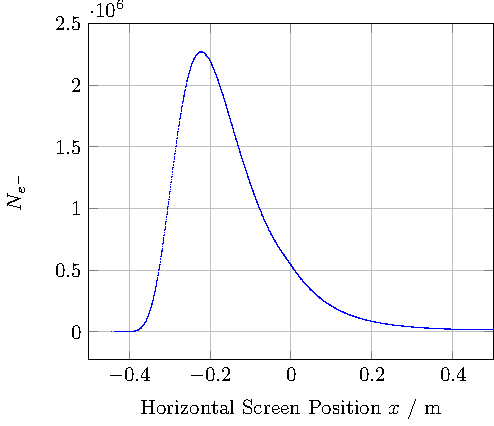
\includegraphics[width=1\linewidth]{./figures/edist.pdf}
	\includegraphics{./output/run-pespread/emitperr_vs_pespread.pdf}
	\caption{
	}
	\label{fig:emitperr_pespread}
\end{figure}


Initially, the mean energy of the beam and energy spread of the beam were tested
independently. Simulations for all combinations of the following energies \(E
\in \left\{ 0.5, 1, 1.3, 2.0, 3.0 5.0\right\} \) and the following energy
spreads \(\sigma_E \in \left\{ 0.01, 0.1, 0.3, 0.4 \right\}\) were run.  These
energies and energy spreads were chosen such that at least one standard
deviation of the beam hit the screen. As Figure~\ref{fig:eofx} shows, the range
of energies that hit the screen for the is from
\SIrange{\sim0.28}{6}{\giga\electronvolt}.

The estimated energy spread of the electron beam is
\SI{0.4}{\giga\electronvolt}, 
% TODO dipole adjustable so could have larger energies
% TODO still need to investigate upper range



It was found that the error of the measurement of the emittance 
% TODO oh god this was the wierd one

Mean beam energies tested ranged from \SIrange{0.1}{4}{\giga\electronvolt}

\subsection{Input Emittance}

\begin{figure}[!tb]
	\centering
		\centering
		\includegraphics{./output/run-inemit/emitr_vs_inemit.pdf}
		\caption{
		}
		\label{fig:emitr_inemit}
\end{figure}

\begin{figure}[!tb]
	\centering
		\centering
		\includegraphics{./output/run-inemit/emitrperr_vs_inemit.pdf}
		\caption{
		}
		\label{fig:emitrperr_inemit}
\end{figure}

\begin{figure}[!tb]
	\centering
	\includegraphics[width=\columnwidth]{./output/run-inemit/emit_7e-5/n1/graph.pdf}
	\caption{
		Beam reconstruction for a large beam emittance of \SI{7e-5}{\meter\radian}
		showing the underestimation of the measured vertical beam sizes.
	}
	\label{fig:large_emit}
\end{figure}

Since the emittance is the variable to be measured, a reasonably large region
around the expected emittance should give presice emittance measurements. The
input beam emittance range tested was from \SIrange{1e-7}{1e-4}{\meter\radian}
with all other parameters kept constant.

\subsection{Background Photons}


\begin{figure}[!t]
	\centering
	\includegraphics{./output/run-bgdens/emit_vs_bgdens.pdf}
	\caption{
	}
	\label{fig:emit_bgdens}
\end{figure}
\begin{figure}[!t]
	\centering
	\includegraphics{./output/run-bgdens/emitperr_vs_bgdens.pdf}
	\caption{
	}
	\label{fig:emitperr_bgdens}
\end{figure}

\begin{figure}[!tb]
	\centering
	\includegraphics[width=\columnwidth]{./output/run-bgdens/bgphotons_1e4/n6/graph.pdf}
	\caption{
		Beam reconstruction for a large background.
	}
	\label{fig:large_bg}
\end{figure}





\section{Conclusion}
\label{sec:conclusion}

% !!! TODO conclusion
The effect of three different experimental parameters were investigated, and
the ranges between which the emittance measurements were accurate and reasonably
precice were found. Despite the fact that the error measurements were
misscalculated, these can be infered from the spread of these measurements.
So the behaviour of the emittance measurement with respect to these parameters
have been presented.

There still remains many 


% 
% % \appendix
% \begin{appendices}
% \part{Code}
% \end{appendices}


\bibliographystyle{ieeetr}
\bibliography{references}

\end{document}

